\chapter{Estado de la Cuestión}
\label{cap:estadoDeLaCuestion}

\begin{resumen}
	En este capítulo estudiaremos las distintas bases de datos que podemos utilizar, así como los modelos que ya hay.
\end{resumen}

\section{Electrocardiogramas}
Un electrocardiograma es una prueba médica en la que se mide la diferencia de potencial entre varios puntos del cuerpo (cada diferencia de potencial recibe el nombre de derivación). Para hacer un ECG estándar, se ponen diez electrodos en puntos concretos del cuerpo y se generan doce ondas que representan la diferencia de potencial entre doce pares de estos electrodos.

Como es natural, no podemos tomar una cantidad continua de medidas del cuerpo, así que los electrocardiogramas funcionan a una frecuencia específica, lo que indica el número de muestras numéricas que toma el aparato medidor por segundo. Lo estándar es que los electrocardiogramas se tomen a 100Hz o a 500Hz dependiendo de la calidad del aparato medidor.

Con estas gráficas (podemos ver los datos de un electrocardiograma extraido de \cite{ptbxldb} y dibujado mediante la librería de python \emph{ecg\_plot} en la Figura \ref{fig:ecg12}), un médico puede detectar alteraciones en el ritmo cardíaco que indiquen diferentes patologías cardíacas.

Por tanto, la información de un electrocardiograma puede almacenarse simplemente en doce vectores de tamaño $100$ o $500$ por segundo de duración del ECG. Estos son los datos con los que funcionan los modelos de predicción actuales. Nosotros utilizaremos la transformada de Fourier de tiempo reducido (o, por sus siglas en inglés, \textbf{STFT}) para crear una imagen (osea, una matriz) a partir de cada una de las doce derivaciones. Luego entrenaremos modelos ligeramente modificados para clasificar anomalías a partir de estas imágenes u otras transformaciones de las mismas.

\begin{figure}
	\setlength{\fboxsep}{0pt}%
	\fbox{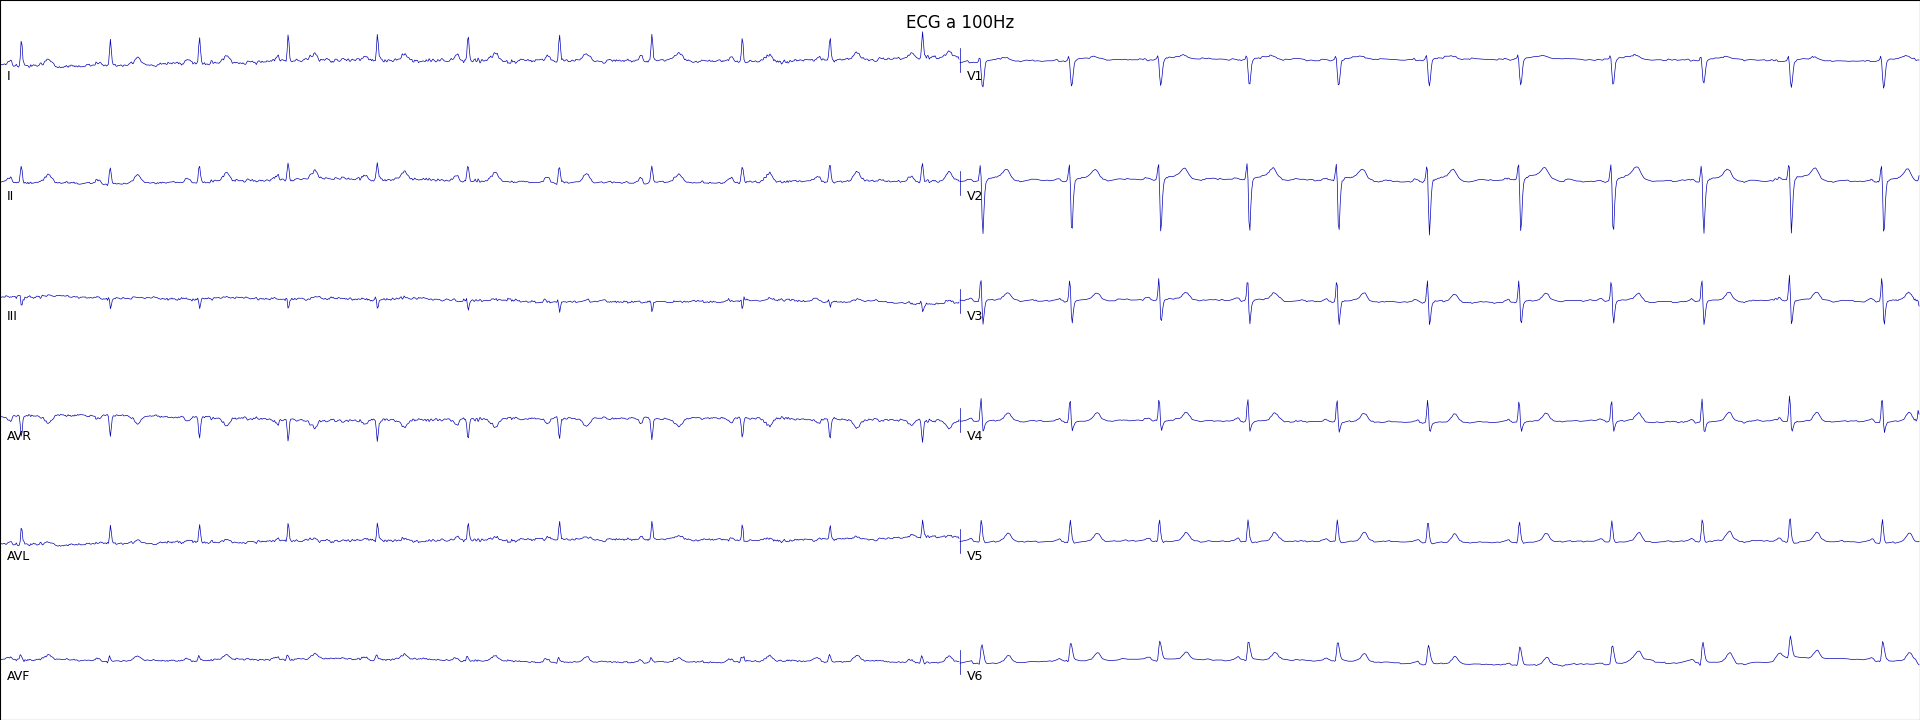
\includegraphics[width=\linewidth]{../Codigo/out/ecg100.png}}
	\fbox{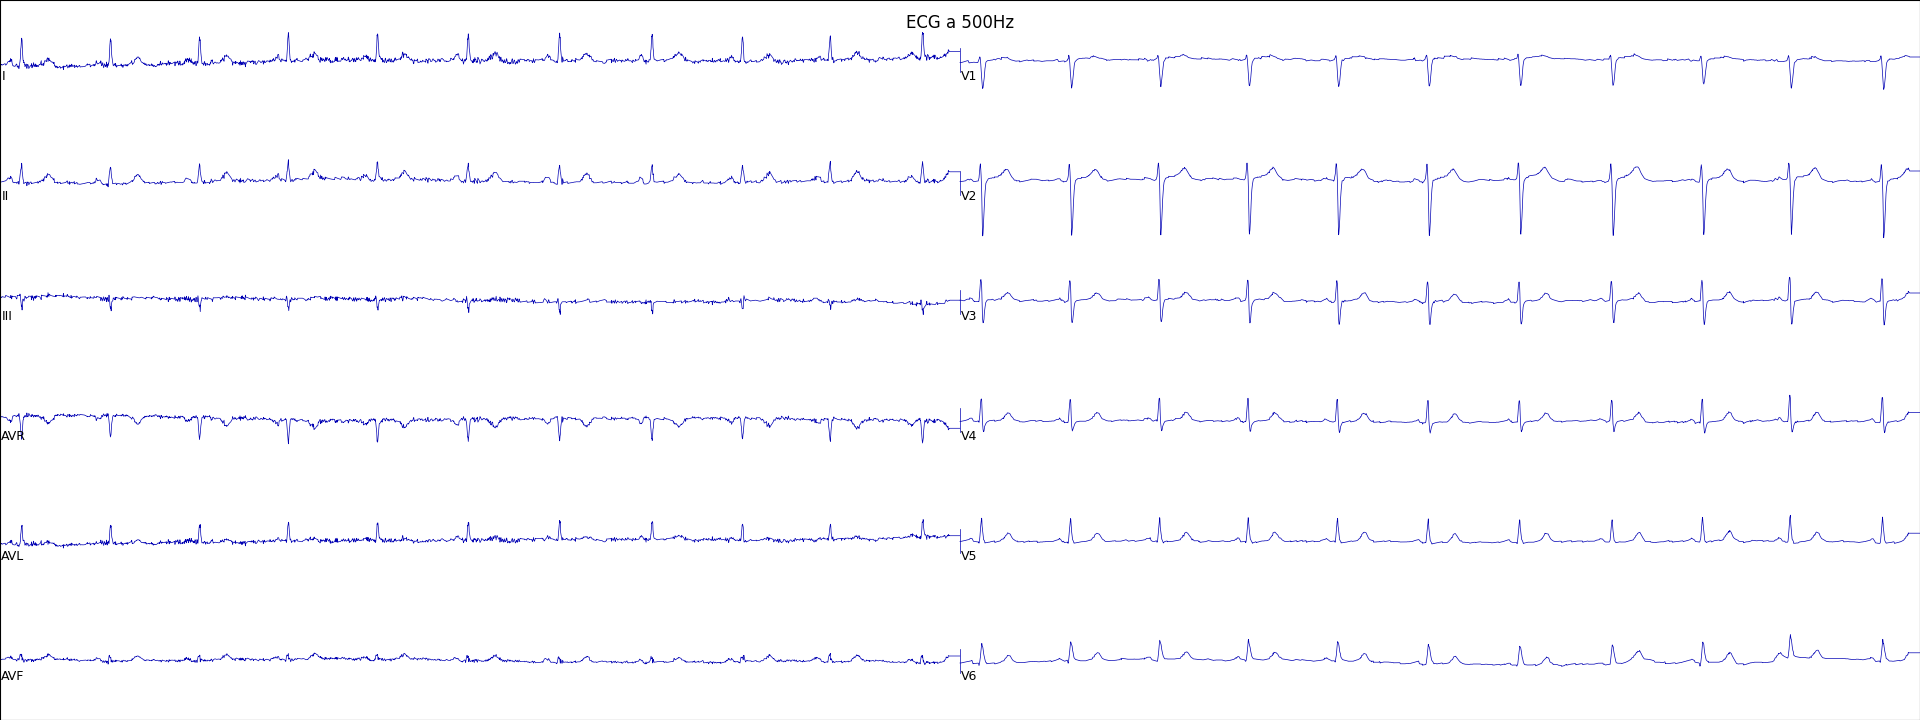
\includegraphics[width=\linewidth]{../Codigo/out/ecg500.png}}
	\caption{Mismo electrocardiograma de 12 derivaciones tomado a 100Hz (arriba) y 500Hz (abajo).}
	\label{fig:ecg12}
\end{figure}

\section{Bases de datos}
Como queremos modificar y comparar el modelo de Ribeiro, lo ideal sería trabajar con la misma base de datos que este para entrenar y probar nuestros modelos, pero esta base de datos, llamada CODE \citep{code}, no es pública, por lo que esto no es una opción.

Existe una versión pública reducida de la base de datos llamada CODE-15 \citep{code15}, que tiene al rededor de $350000$ casos. No obstante, no podemos comparar un modelo entrenado con los datos de CODE-15 con otro entrenado con los datos originales, porque la ventaja en el conjunto de datos de entrenamiento haría imposible comparar la eficiencia y explicabilidad de manera equitativa. Por ello, vamos a volver a entrenar el modelo original de Ribeiro con una base de datos pública.

No obstante, en lugar de entrenar todos nuestros modelos con CODE-15, utilizaremos otra base de datos completamente pública, la PTB-XL \citep{ptbxldb}. Esta base de datos cuenta solo con unos $22000$ casos de prueba, pero todos estos casos vienen con el mismo formato, por lo que procesar los datos va a ser mucho más sencillo con esta base de datos. Además, dado que el objetivo es comparar si las modificaciones de los modelos mejoran el rendimiento, es mucho más importante que las bases de datos sean iguales y poder hacer varios entrenamientos que utilizar una base de datos enorme con la que nos lleve mucho más tiempo entrenar los modelos.

Un posible trabajo futuro sería escoger el modelo que mejor nos haya funcionado y volver a entrenarlo con una base de datos mayor (incluso con CODE si se tuviera acceso a ella), y luego compararla con el modelo de Ribeiro original, no obstante, eso queda fuera del alcance de este documento.

\section{Modelos}
Como hemos mencionado ya varias veces, el modelo que nos va a servir de referencia en este trabajo es el de Ribeiro, por ser el que mejores resultados ha obtenido hasta ahora. No obstante, también probaremos con otros modelos.

En concreto, existe una modificación del modelo de Ribeiro que, con tan solo 3 derivaciones, consigue unos resultados muy parecidos \citep{TFGSergio}. Además, este modelo tiene la ventaja de estar ya entrenado con los datos de PTB-XL, por lo que no haría falta volver a entrenar el modelo original.